\chapter{Graph-Theoretic Foundation}
\label{ch:graph}
\section{Introduction}
The purpose of this chapter is to motivate the use of the \ac{MCMM} as Multimorph's learning framework. The key concept in this chapter will be the \emph{bipartite} graph, a type of graph so named because its nodes can be partitioned into two subsets according to criteria which we shall discuss below. This chapter will maintain that bipartite graphs have properties that are essential to the tasks of modeling and learning non-concatenative morphology.
% a type of graph with two sets of nodes such that only nodes of different sets are connected. Within each set, there are no connections. This intra-layer independence engenders some important properties, as we shall see.
We shall begin in section~\ref{sec:bipartite} by introducing the mathematical concept of the \emph{bipartite graph}, placing particular importance on the properties that make this type of graph naturally conducive to modeling non-concatenative morphology. %We shall demonstrate that bipartite graphs are essential for the modeling of nonconcatenative morphology (and thus morphology in general). 

In section~{sec:autoseg-bipart} we shall take a fresh look at McCarthy's autosegmental framework for morphology \citep{mccarthy:1981} in light of the properties of the bipartite graph. We shall thus see that not only is McCarthy's framework itself bipartite graph, but that the properties of bipartite graphs are essential for the modeling of non-concatenative morphology.
% naturally well-suited to modeling non-concatenative morphology. and more than that, we will argue that bipartite graphs are general that ultimately derive from these properties two necessary conditions that morphological models must satisfy in order to be capable of modeling bipartite graphs two criteria that a morphological model must satisfy We will see that McCarthy's framework is itself a bipartite graph. and re
Finally, in section~\ref{mcmm-bipart}, we point out that an \ac{MCMM} is a bipartite graph, and that, consequently, it is compatible so to  speak with autosegmental morphology. In other words, an MCMM can serve as a
a computational ``wrapper," so to speak, for McCarthy's autosegmental theory, a means whereby it can be specially packaged for use in a machine learning system. 
 
%itself has a bipartite architecture, which is to say that it can be represented as and thought of as a bipartite graph without information loss.  essentially bipartite in its architecture, and that it ; we will see that the autosegmental framework is essentially a bipartite graph. We shall then observe in section~\ref{sec:mcmm-bipart} that an \ac{MCMM} is itself a bipartite graph, and that autosegmental morphology and \ac{MCMM}s have the same graphical properties. From this point, the conclusion follows that an From a theoretical perspective, therefore, it is a sound choice to use the \ac{MCMM} as a computational``wrapper," as it were, for McCarthy's theoretical autosegmental framework, to package for it for use a machine learning system. 
%The argumentation in this chapter will proceed as follows: 
%\begin{enumerate}
%\item We shall first demonstrate that the autosegmental morphological framework of \cite{mccarthy:1981} is, in its essence, a bipartite graph.
%\item We shall then observe that an \ac{MCMM} is quite clearly a bipartite graph. 
%\item From these two points, it follows that autosegmental morphology and \cm
%\end{enumerate}

%We shall first show that McCarthy's autosegmental morphological framework of \cite{mccarthy:1981} is a bipartite graph. We we shall show that an MCMM is a bipartite graph. And connecting the latter point to the former, %the latter point to the former, 
%we shall conclude that because the MCMM and McCarthy's autosegmental formalism 
%are both bipartite graphs, the MCMM is a very appropriate learning framework for 
%modeling autosegmental morphology and thus for learning nonconcatenative 
%morphology. The \ac{MCMM}, therefore, is well-suited to serve as a computational implementation of autosegmental morphology. %mathematically, and in particular, graph-theoretically. , we shall introduce the \emph{multipartite graphs}, 
%particularly \emph{bipartite graphs}, as well as discuss their relationship to autosegmental morphology, and hence their significance to the problem of
%learning non-concatenative morphology.   
%relevance to the problem of leand their relationship 
%to autosegmental morphology.
% which are a subset, i.e., special case, of multipartite graphs. 
\section{Bipartite Graphs}\label{sec:bipartite}
A \emph{multipartite} graph is a graph 
whose nodes can be partitioned into $N$ disjoint sets of 
\emph{mutually nonadjacent} nodes, i.e., $N$ sets such that no two
nodes within the \emph{same} set are connected by an edge. A bipartite graph
is simply multipartite graph such that $N = 2$. Thus, a bipartite graph is defined 
as in \ref{ex:bipartite}: 
%graph that satisfies the following: i.e., it has two partitions of nodes  That is, a graph is \textbf{bipartite} if it satisfies the following
%criteria in \ref{ex:bipartite}.
%\begin{definition} A graph is \textbf{bipartite} if it satisfies the following criteria:
%\begin{enumerate}
%\item The graph's nodes are separated into two disjoint sets (or partitions).
%\item Within each partition, all nodes are independent, i.e., mutually nonadjacent.
%\end{enumerate}
\begin{exe} \label{ex:bipartite} \ex A \textbf{bipartite} graph is a graph in which:\begin{xlist} 
	\ex %{\textsc{Nonlinearity}}.  %A model is \emph{nonlinear} 
	the nodes divided into two disjoint sets, or partitions. \label{ex:bipartite1} %separated into two disjoint sets, or partitions. %eparately for m  as being separate from (or outside of) the the phonological (or segmental) tier.  % is a property wherein morphs are represented as being separate from the segmental tier.
	\ex %Within each partition, nodes are mutually non-adjacent. % ; 
	Two nodes are members of the same partition if and only if 
	they are \emph{not} connected by an edge.
	\label{ex:bipartite2}
	\end{xlist}
\end{exe}
%\end{definition}
(i.e., non-adjacent). Conversely, 
	if two nodes \emph{are} connected (or adjacent), they necessarily belong to different sets. 
	\emph{This means that \textbf{within} each or partition, all nodes are independent 
	(i.e., not connected).}
These two criteria are equivalent to the properties of nonlinearity and 
nonsequentiality, respectively, first defined in chapter~\ref{ch:intro}.

\section{Autosegmental Morphology is Bipartite}\label{sec:autoseg-bipart}
The central aspect of autosegmental theory 
is its \emph{multi-linear} architecture, i.e., its use of a 
\emph{segmental tier} along with many \emph{autosegmental tiers} to 
account for the surface forms of words\ cite{mccarthy:1981}. The segmental tier is home to the sequence of consonants and vowels that define the linear arrangement of phonological features. Each autosegmental tier is home to a morph. Each morph, therefore, occupies its own distinct plane and is thus external to the segmental tier. The separation of morphs from the segmental tier allows a given morph to connect to nonadjacent phonological segments, as illustrated in figure~\ref{subfig:multilinear}. %as well as from each other gives rise to a multi-linear architecture. 
The multi-linear architecture of autosegmental theory thus provides a means of
dealing with nonconcatenative morphology. 

One can see this plainly by comparing figures~\ref{subfig:multilinear} and \ref{subfig:linear}. Each shows an attempt to analyze the word \emph{hizkir} `he reminded', in which the root \textit{z-k-r} (morph $\mu_3$) is interrupted by the /i/ of morph $\mu_2$ and is thus a discontinuous, or non-concatenative morph. Figure~\ref{subfig:multilinear} is a multilinear autosegmental approach (or nonlinear nonsequential type of model described in chapter~\ref{ch:LitReview}), whereas figure~\ref{subfig:linear} is a linear approach. The multilinear approach is able to recognize the root \textit{z-k-r} as a coherent morph despite its discontinuity. The linear approach, by contrast, has no way to group the \textit{r} with the \textit{z} and {k}.

In figure~\ref{subfig:multilinear}, we see at work the properties \emph{nonlinearity} and \emph{nonsequentiality}, first defined in chapter~\ref{ch:lit-review}.
Let us restate these properties here as (\ref{ex:criteria1-again}) and (\ref{ex:criteria2-again}).
\begin{exe} \label{ex:criteria-again} \ex \begin{xlist}
	\ex {\textsc{Nonlinearity}}.  %A model is \emph{nonlinear} 
	Morphs must be separate from the phonological tier. \label{ex:criteria1-again}
%	Morphs must be represented separately 
%	from the surface (or phonological) tier, i.e., as residing on tiers distinct from 
%	the phonological tier. \label{ex:criteria1-again}%eparately for m  as being separate from (or outside of) the the phonological (or segmental) tier.  % is a property wherein morphs are represented as being separate from the segmental tier.
	\ex {\textsc{Nonsequentiality}}.
	Each morph tier must be orthogonal to all other morph tiers. \label{ex:criteria2-again}
	%Each morph tier is required to be orthogonal to all other morph tiers. \label{ex:criteria2-again}
	\end{xlist}
\end{exe}

%	\begin{definition}\label{def:nl}{\textsc{Nonlinearity}}: %A model is \emph{nonlinear} 
%	Morphs must be separate from the phonological tier. \end{definition}
%	%Morphs, i.e., units of morphological structure, must be separate from the surface (or phonological) tier. \end{definition} %, i.e., as residing on tiers distinct from the phonological tier. %eparately for m  as being separate from (or outside of) the the phonological (or segmental) tier.  % is a property wherein morphs are represented as being separate from the segmental tier.
%	\begin{definition}\label{def:ns}{\textsc{Nonsequentiality}}: %is a property such that each morph tier (or node) is orthogonal to all other morph tiers.
%	%---i.e., independent of---all other morph tiers. 
%	Each morph tier must be orthogonal to all other morph tiers.
%	\end{definition}
%\begin{proposition}\label{prop:nlns}
%A model of morphology can handle nonconcatenative morphology if and only if it satisfies both \textbf{nonlinearity} and \textbf{nonsequentiality}. %  the modeling of nonconcatenative morphology.}
%\end{proposition}
%\pex~ Two essential properties  %\ex \label{ex:properties}\begin{xlist}
%	\a {\textsc{Nonlinearity}}: Morphemes are represented as being separate from the segmental tier.
%	\a {\textsc{Nonsequentiality}}: Each morpheme tier (or node) is orthogonal to---i.e., independent of---all other morpheme tiers.
%\xe
% \ex this is one 
%\marginpar{or multilinear}

%and comprises one or more (not necessarily contiguous) feature bundles. Each feature bundle can associate with any phonological segment in the \emph{segmental tier} as long as the association lines of  
%In chapter~\ref{ch-Intro}, I stated that 
%Recall that one of this dissertation's primary objectives is to implement autosegmental morphology computationally, so that it might equip an unsupervised machine learning system to learn non-concatenative morphology, 
There is a clear correspondence between these two properties  %(\ref{ex:criteria1-again}) (\ref{ex:criteria2-again})  
and the two components of the definition of \emph{bipartite} in (\ref{ex:criteria-again}).
The reason for this correspondence is that the autosegmental framework is essentially a bipartite graph. 
We can make this clearer simply be rearranging the morph nodes $\mu_1$, $\mu_2$, and $\mu_3$. That is, can simply move up $\mu_2$ so that it is situated between $\mu_1$ and $\mu_3$, i.e., so that all three morphs are lined up in a row. We can then regard this row (or vector) of morphs as one of the partitions in a bipartite graph. The segmental tier would constitute the other partition. And since all components in a vector are orthogonal to one another, the morph in a vector of morphs can still be regarded as residing on different tiers. %This would not effect the indpendence of th mo
%in order to enable this system
% Explored in linguistic theory and computationally with hand-written grammars ...
%to learn nonconcatenative morphology without supervision. 
%in a machine learning system capable of learning nonconcatenative morphology without supervision.
%During the course of development, I will explore different options for system components, e,g., the set of features,
%in order to arrive at the configuration that gives the best result for learning autosegmental morphology.  

%0. Already accepted as fact/Already proposed/hypothosized. Isolate the aspect(s) of AT that are responsible 
%for its ability to deal with nonconcatenative morphology.
%\cite{mccarthy:1981} has shown that it is the multi-linear architecture of autosegmental theory that allows it to deal with
%nonconcatenative morphology. 
%In graph theoretic terms, this multi-linear formalism constitutes a \emph{multipartite}, or $K$-partite, graph,
%i.e., a graph whose nodes form $K$ sets of \emph{mutually nonadjacent} nodes. That is, there are no edges between nodes of the same set, but there may be an edge betwech-Introen edges of different sets. 

%In an autosegmental representation, each tier, or morpheme, 
%is a set of mutually nonadjacent nodes, where   
%each node is a distinct bundle of phonological features.
%But note that each morpheme tier can be represented abstractly as a single node; that is, 
%its component nodes need not be represented explicitly 
%because they are given by the edges linking the morpheme to the phonological segments.
We can thus view all the morpheme tiers as composing a single tier, with each morpheme represented as a single node in this tier.
We will call this morpheme tier the \emph{hidden} \emph{layer}, the segmental tier the \emph{surface} \emph{layer}. 
In this way, the autosegmental multi-linear framework can be represented as a bipartite graph.

%This bipartiteness is important because many learning algorithms are based on bipartite graphs. I will be focusing on one such algorithm called
%the Multiple Cause Mixture Model (MCMM)
%\citep{saund:94}. An MCMM is a kind of autoencoder network with a bipartite architecture. It has two layers of nodes, a reconstruction (surface) layer $R$, where it attempts to reconstruct the input feature vectors and a hidden layer whose nodes encode shared features among the input vectors. Weighted arcs link the nodes of one layer to those of the other, but there are no \emph{intra}-layer connections.

% Hebrew morphology, both its non-concatenative and concatenative components. 
%In a multi-linear framework, concatenative morphology is just a special case of non-concatenative morphology. There is no fundamental difference between them.

\begin{figure}%{ht}
%\vspace{-20pt}
	\centering
	\subfigure[Multilinear approach]{
	\begin{tikzpicture}[shorten >=1pt,draw=black!100]
	\def \rowtwoht{5cm}
	%\def \weightstwo{3.75cm}
	\def \rowoneht{3.5cm}
	%\def \weightsone{1.25cm}
	\def \basement{2cm}
	\tikzstyle{m-node}=[text height=6pt,text centered,inner sep=6pt,minimum size=15pt]
	\tikzstyle{r-node}=[text height=6pt,text centered,inner sep=6pt,minimum size=15pt]
	\tikzstyle{d-node}=[text height=6pt,text centered,inner sep=6pt,minimum size=15pt]
	\tikzstyle{annot}=[text width=20ex]
	% labels
	\node[annot] (mtierstop) at (0cm,\rowtwoht) {};
	\node[annot] (segtier) at (0cm,\rowoneht) {surface layer};
	\node[annot] (mtiersbot) at (0cm,\basement) {};
	
	% hidden layer
	\node[m-node] 	(m0)	at (1.7cm,\rowoneht)		{h};
	\node[m-node] 	(m1)	at (2.0cm,\rowoneht)		{i};
	\node[m-node] 	(m2)	at (2.3cm,\rowoneht)		{\textbf{z}};
	\node[m-node] 	(m3)	at (2.6cm,\rowoneht)	 	{\textbf{k}};
	\node[m-node] 	(m4)	at (2.9cm,\rowoneht)	 	{i};
	\node[m-node] 	(m5)	at (3.2cm,\rowoneht)	 	{\textbf{r}};
	
	% reconstructed vector
	\node[r-node] 	(r0)	at (2.3cm,\rowtwoht)		{$\mu_{1}$};
	%\node[r-node] 	(r6) 	at (9.75cm,\rowoneht)   	{$r_J$};
	
	% data vector
	\node[d-node] 	(d0)	at (1.8cm,\basement)		{$\mu_{2}$};
	\node[d-node] 	(d1)	at (2.9cm,\basement)		{$\mu_{3}$};
	%\node[d-node] 	(d6) 	at (9.75cm,\basement)   	{$d_J$};
	
	\path
		(r0)	edge	node	{}	(m2)
		(r0)	edge	node	{}	(m3)
		(r0)	edge	node	{}	(m5)
		%
		(d0)	edge	node	{}	(m0)
		(d0)	edge	node	{}	(m1)
		(d1)	edge	node	{}	(m4);
		
	\end{tikzpicture}
	\label{subfig:multilinear}

	}
	\subfigure[Linear approach]{
	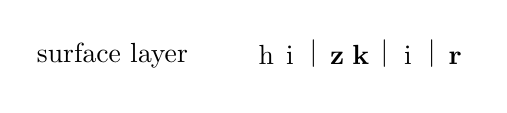
\begin{tikzpicture}[shorten >=1pt,draw=black!100]

	\def \floor{0cm}
	\tikzstyle{f-node}=[text height=6pt,text centered,inner sep=6pt,minimum size=15pt]
	\tikzstyle{annot}=[text width=20ex]
	% labels
	\node[annot] (floorlabel) at (0cm,\floor) {surface layer};
	
	% surface layer
	\node[f-node] 	(f0)	at (1.4cm,\floor)		{h};
	\node[f-node] 	(f1)	at (1.7cm,\floor)		{i};
	\node[f-node] 	(f2)	at (2cm,\floor)		{$|$};
	\node[f-node] 	(f3)	at (2.3cm,\floor)		{\textbf{z}};
	\node[f-node] 	(f4)	at (2.6 cm,\floor)	 	{\textbf{k}};
	\node[f-node] 	(f5)	at (2.9 cm,\floor)	 	{$|$};
	\node[f-node] 	(f6)	at (3.2 cm,\floor)	 	{i};
	\node[f-node] 	(f7)	at (3.5 cm,\floor)	 	{$|$};
	\node[f-node] 	(f8)	at (3.8 cm,\floor)	 	{\textbf{r}};
	\end{tikzpicture}
	\label{subfig:linear}
	}
\caption{Two approaches to analyzing \textit{hizkir} (`he reminded'), which has three morphemes. 
The root \textit{z-k-r} (boldface) is discontinuous. The linear (single-tier) approach is unable to connect the \textit{r} to the \textit{zk}, while the multilinear approach is able to unite discontiguous elements through external morpheme ($\mu$) nodes.}
%: an input layer ($\mathbf{d}$), a hidden layer ($\mathbf{m}$), and an output layer
\label{fig:approaches}
\end{figure}

% Describe how autosegmental theory reduces to a bipartite graph. 
In an autosegmental representation, each morph tier is a complex object, consisting of a particular sequence of phonological feature matrices, e.g., [-front,+low,-round,+syllabic]. However, one can generally use phonemic symbols as shorthand for
feature matrices; e.g., the feature matrix [-front,+low,-round,+syllabic] can be written as \textipa{/a/}. A sequence of feature matrices can thus be reduced to a sequence of alphabetic characters, each of which represents a particular set of features. For example, in figure~\ref{subfig:multilinear}, one morph is represented as the sequence \textipa{/hi/}, which is an abbreviation of \textipa{/}[+spread glottis][+front,-low,-round,+syllabic]\textipa{/}.
When feature matrices represented by /h/ and /i/ become linked to the first C and the first V, respectively, the C and V inherit these same feature matrices, which means that /h/ and /i/ can now also stand in for the initial C and V (respectively). 

A CV skeleton becomes a sequence of fully fledged phonemes, i.e., a phonological
form, as soon as morph tiers connect to its C and V slots, and it does so by taking 
on the identities of the phonological elements that compose the morphs. 
Thus, just as \textipa{/hi/} and \textipa{/i/} (i.e, the feature bundles they represent) compose 
$\mu_1$ in figure~\ref{subfig:multilinear}, they also now compose a morphological 
unit within the segmental tier. The morphs $\mu_1$, $\mu_2$, and $\mu_3$ 
essentially \emph{cause} the segmental tier to be realized as a fully fledged 
phonological form. These observations with become particular relevant in section~\ref{sec:mcmm-bipart} 
below as the following chapter, for we are coming close to describing the workings 
of \ac{MCMM}. 

%One might thus object to the simplicity of figure~\ref{subfig:multilinear}, e.g., its denoting the autosegmental morph tiers as $mu1$, etc., as though they were atomic units. But these labels are merely a form of shorthand. That is, one can generally use phonemic symbols as shorthand for
%feature matrices; e.g., the feature matrix [+back,+low, -cons] can be written as /a/
%%is a set of mutually nonadjacent nodes, where   
%each node is a bundle phonological features, e.g., [+back,+low, +syllabic]. However, one can generally use phonemic symbols as shorthand for
%feature bundles (or matrices); e.g., the feature matrix [+back,+low, +syllabic] can be written as /a/. 
%as  

These features are mapped onto the
C and V slots in McCarthy's segmental tier. 
 Each node, therefore, is complex.
But note that each morpheme tier can be represented abstractly as a single node; that is, 
its component nodes need not be represented explicitly 
because they are given by the edges linking the morpheme to the phonological segments.
We can thus view all the morpheme tiers as composing a single tier, with each morpheme represented as a single node in this tier.
We shall call this morph tier the \emph{hidden} \emph{layer}, the segmental tier the \emph{surface} \emph{layer}. 
In this way, the autosegmental multi-linear framework can be represented as a bipartite graph.

For convenience, we restate these properties here as (\ref{ex:criteria1-again}) and (\ref{ex:criteria2-again}):
\begin{exe} \label{ex:criteria-again} \ex \begin{xlist}
	\ex {\textsc{Nonlinearity}}.  %A model is \emph{nonlinear} 
	Morphs must be represented separately 
	from the surface (or phonological) tier, i.e., as residing on tiers distinct from 
	the phonological tier. \label{ex:criteria1-again}%eparately for m  as being separate from (or outside of) the the phonological (or segmental) tier.  % is a property wherein morphs are represented as being separate from the segmental tier.
	\ex {\textsc{Nonsequentiality}}.
	Each morph tier is required to be orthogonal to all other morph tiers. \label{ex:criteria2-again}
	\end{xlist}
\end{exe}
Fig.~\ref{fig:bipartite} is a bipartite
graph; its nodes are divided into two partitions, namely the sets $M$
and $R$. Within each set, all nodes are independent; 
the only connections are between nodes of different sets.

In graph-theoretic terms, the multi-linear formalism of
\cite{mccarthy:1981} is a type of \emph{multipartite}
graph. This is a graph whose nodes can be partitioned into two sets whose members are \emph{mutually nonadjacent}; i.e., no two nodes within the same set are connected by an edge.
%\emph{mutually nonadjacent}, i.e., disconnected, nodes; i.e., there are no connections between nodes of the same set. %two sets such that whose defining characteristic is that no two nodes with
%nodes within the \emph{same} set are connected by an edge.
Fig.~\ref{fig:bipartite}, for example, shows a \emph{bipartite}
graph, i.e., a graph with two such partitions, namely the sets $M$
and $R$ in this case.
Within each set, or \emph{layer}, all nodes are independent; that is there are no
intra-layer connections. The only connections are 
between nodes of different sets.

 \begin{figure}[htb]
 \begin{center}
 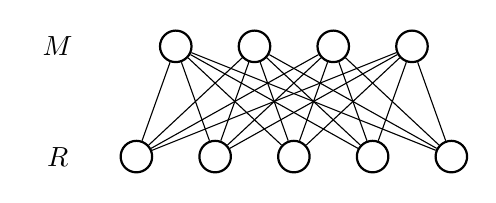
\begin{tikzpicture}[draw=black!100,scale=1.0]
 	\def \rowtwoht{1.4cm}
 	\def \rowoneht{0.0cm}
 	\tikzstyle{m-node}=[circle,draw=black!100,thick,inner sep=0pt,minimum size=4mm]
 	\tikzstyle{r-node}=[circle,draw=black!100,thick,inner sep=0pt,minimum size=4mm]
 	\tikzstyle{annot} = [text width=1.5em, text centered]
 	\node[annot] (hidden-label) at (-0.5cm,\rowtwoht) {$M$};
 	\node[annot] (surface-label) at (-0.5cm,\rowoneht) {$R$};
 	\node[m-node] 	(m0)	at (1cm,\rowtwoht)		{};
 	\node[m-node] 	(m1)	at (2cm,\rowtwoht)		{};
 	\node[m-node] 	(m2)	at (3cm,\rowtwoht)	 	{};
 	\node[m-node] 	(m3)	at (4cm,\rowtwoht) 		{};
 	% surface layer
 	\node[r-node] 	(r0)	at (0.5cm,\rowoneht)		{};
 	\node[r-node] 	(r1)	at (1.5cm,\rowoneht)		{};
 	\node[r-node] 	(r2)	at (2.5cm,\rowoneht)	 	{};
 	\node[r-node] 	(r3)	at (3.5cm,\rowoneht) 		{};
 	\node[r-node] 	(r4) 	at (4.5cm,\rowoneht)   		{};
 	%\node[r-node] 	(r5) 	at (6.5cm,\rowoneht)   		{};
 	\path (r0)	edge	node	{}	(m0)
		(r0)	edge	node	{}	(m1)
		(r0)	edge	node	{}	(m2)
		(r0)	edge	node	{}	(m3)

		(r1)	edge	node	{}	(m0)
		(r1)	edge	node	{}	(m1)
		(r1)	edge	node	{}	(m2)
		(r1)	edge	node	{}	(m3)

		(r2)	edge	node	{}	(m0)
		(r2)	edge	node	{}	(m1)
		(r2)	edge	node	{}	(m2)
		(r2)	edge	node	{}	(m3)
						
		(r3)	edge	node	{}	(m0)
		(r3)	edge	node	{}	(m1)
		(r3)	edge	node	{}	(m2)
		(r3)	edge	node	{}	(m3)

		(r4)	edge	node	{}	(m0)
		(r4)	edge	node	{}	(m1)
		(r4)	edge	node	{}	(m2)
		(r4)	edge	node	{}	(m3);
 		%(m3)	edge	node	{}	(r5);		
 \end{tikzpicture}
 \end{center}
 \caption{Bipartite graph}
 %. Neither layer contains sequential dependencies; every unit is independent within its own layer. Each hidden unit is thus free to cause any combination of observed units.}
 \label{fig:bipartite}
 \end{figure}

%This bipartiteness is important because many learning algorithms are based on bipartite graphs. I will be focusing on one such algorithm called
%the Multiple Cause Mixture Model (MCMM)
%\citep{saund:94}. An MCMM is a kind of autoencoder network with a bipartite architecture. It has two layers of nodes, a reconstruction (surface) layer $R$, where it attempts to reconstruct the input feature vectors, and a hidden layer whose nodes encode shared features among the input vectors. Weighted arcs link the nodes of one layer to those of the other, but there are no \emph{intra}-layer connections.

% Hebrew morphology, both its non-concatenative and concatenative components. 
%In a multi-linear framework, concatenative morphology is just a special case of non-concatenative morphology. There is no fundamental difference between them.
\section{An MCMM is a Bipartite Graph}\label{sec:mcmm-bipart}
An MCMM, as it turns out, is a special case of a bipartite graph. Indeed,
fig.~\ref{fig:bipartite} could itself be a simple MCMM. %precisely the architecture of an MCMM.
%To sum up, bipartite graphs possess the properties nonlinerarity and nonsequentiality. 
Because MCMMs are bipartite graphs, and bipartite graphs are both nonlinear and nonsequential, 
MCMMs must themselves be nonlinear and nonsequential, which makes MCMMs well-suited for modeling
non-concatenative morphology.

%As it turns out, 
A bipartite graph suffices
%we do not need many partitions 
to capture the essential properties of McCarthy's autosegmental
framework,
% (fig.~\ref{subfig:nonlinear}). 



\section{Conclusion}
\label{sec:mcmm-bipart}

That is, because of its bipartite properties, an MCMM provides a sound framework in which to implement autosegmental morphology, or at least the components of autosegmental morphology that address non-concatenative morphology.
An MCMM, as it turns out, is a special case of a bipartite graph. Indeed,
fig.~\ref{fig:bipartite} could itself be a simple MCMM. %precisely the architecture of an MCMM.
%To sum up, bipartite graphs possess the properties nonlinerarity and nonsequentiality. 
Because MCMMs are bipartite graphs, and bipartite graphs are both nonlinear and nonsequential, 
MCMMs must themselves be nonlinear and nonsequential, which makes MCMMs well-suited for modeling
non-concatenative morphology.

Because a bipartite graph meets the two criteria stated in
(\ref{ex:criteria}).  We can reformulate the morpheme tiers and the
segmental tier in fig.~\ref{subfig:nonlinear} as the sets $M$ and
$R$, respectively, in fig.~\ref{fig:bipartite} This satisfies the first
criterion. For the second, each node in $M$ represents a morpheme (or
morpheme tier), and, by the definition of \emph{bipartite}, the nodes
within $M$ are independent and thus orthogonal.

An MCMM (section~\ref{sec:mcmm}) is well-suited to learn 
non-concatenative morphology because it is bipartite graph. It has two
\emph{layers} (equivalently, sets) of nodes, a hidden layer and a
surface layer---corresponding, respectively, to $M$ and $R$ in
fig.~\ref{fig:bipartite}. There are no intra-layer connections in an
MCMM, only connections between layers.
%, as in any bipartite graph.

We shall henceforth refer to an MCMM's partitions as
\emph{vectors}, i.e., vectors of nodes, and use matrix and vector notation to
describe the components of an MCMM:
In particular, 
uppercase boldface letters will denote matrices, %(e.g., $\mathbf{M}$),
lowercase boldface letters will denote vectors,
% and matrix rows or columns, 
%(e.g., $\mathbf{m}_i$),
and italicized lowercase letters refer to the individual elements
of vectors/matrices. % (e.g., $m_{ik}$).
For example, $m_{i,k}$ is the $k^{\text{th}}$ element in the vector
$\mathbf{m}_i$, which is the $i^{\text{th}}$ row in the $I \times K$ matrix
$\mathbf{M}$. Thus, we shall henceforth write the $M$ and $R$ in
fig.~\ref{fig:bipartite} as $\mathbf{m}$ and $\mathbf{r}$,
respectively (or $\mathbf{m}_i$ and $\mathbf{r}_i$, where $i$ is the
index of the $i^{\text{th}}$ word).